% !TEX root =  ../c3.tex
\section{Methods}
\label{c3:sec:methods}
\subsection{Study Population}
\label{c3:subsec:study_population}
To develop our methodology, we use the data (see Table~\ref{c3:table:1}) of prostate cancer patients from the world's largest AS study called PRIAS~\citep{bokhorst2016decade}. More than 100 medical centers from 17 countries worldwide contribute to the collection of data, utilizing a common study protocol and a web-based tool, both available at \url{www.prias-project.org}. We use data collected over ten years, between December 2006 (beginning of PRIAS study) and December 2016. The primary event of interest is cancer progression detected upon a positive biopsy. The time of cancer progression is interval-censored because biopsies are scheduled periodically. Biopsies are scheduled as per the PRIAS protocol (see Section~\ref{c3:sec:introduction}). There are three types of competing events, namely death, removal of patients from AS based on their observed DRE and PSA measurements, and loss to follow-up. We assume these three types of events to be censored observations. However, our model allows the removal of patients to depend on observed longitudinal data and baseline covariates of the patient. Under the aforementioned assumption of censoring, Figure~\ref{c3:fig:2} shows the cumulative-risk of cancer progression over the study follow-up period.

\begin{table}
\small
\centering
\caption{\textbf{Summary of the PRIAS dataset}. The primary event of interest is cancer progression. A DRE measurement equal to T1c~\citep{schroder1992tnm} indicates a clinically inapparent tumor which is not palpable or visible by imaging, while tumors with $\mbox{DRE} > \mbox{T1c}$ are palpable. IQR: interquartile range.}
\label{c3:table:1}
\begin{tabular}{lr}
\toprule
Data & Value\\
\midrule
Total patients & 5270\\
Cancer progression (primary event) & 866\\
Loss to follow-up (anxiety or unknown) & 685\\
Removal on the basis of PSA and DRE & 464\\
Death (unrelated to prostate cancer) & 61\\
Death (related to prostate cancer) & 2\\
\midrule
Median Age (years) & 70 (IQR: 65--75)\\
Total PSA measurements & 46015\\
Median number of PSA measurements per patient &  7 (IQR: 5--12)\\
Median PSA value (ng/mL) & 5.6 (IQR: 4.0--7.5)\\
Total DRE measurements & 25606\\
Median number of DRE measurements per patient & 4 (IQR: 3--7)\\
$\mbox{DRE} = \mbox{T1c}$ (\%) & 23538/25606 (92\%) \\
\bottomrule
\end{tabular}
\end{table}

\begin{figure}
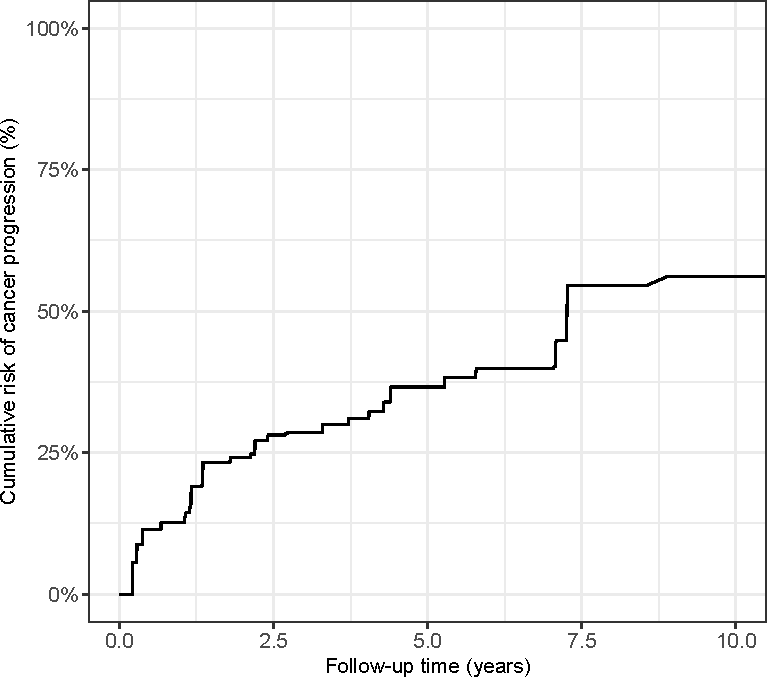
\includegraphics{contents/c3/images/c3_fig2.pdf}
\caption{\textbf{Estimated cumulative-risk of cancer progression in AS} for patients in the Prostate Cancer Research International Active Surveillance (PRIAS) dataset. Nearly 50\% patients (\emph{slow progressing}) do not progress in the ten year follow-up period. Cumulative-risk is estimated using nonparametric maximum likelihood estimation~\citep{turnbull1976empirical}, to account for interval censored cancer progression times observed in the PRIAS dataset. Censoring includes death, removal from AS on the basis of observed longitudinal data, and patient dropout.}
\label{c3:fig:2}
\end{figure}

For all patients, PSA measurements (ng/mL) are scheduled every three months for the first two years and every six months thereafter. The DRE measurements are scheduled every six months. We use the DRE measurements as ${\mbox{DRE} = \mbox{T1c}}$ versus $\mbox{DRE} > \mbox{T1c}$. A DRE measurement equal to T1c~\citep{schroder1992tnm} indicates a clinically inapparent tumor that is not palpable or visible by imaging. In contrast, tumors with $\mbox{DRE} > \mbox{T1c}$ are palpable.

\textbf{Data Accessibility:} The PRIAS database is not openly accessible. However, access to the database can be requested based on a study proposal approved by the PRIAS steering committee. The website of the PRIAS program is \url{www.prias-project.org}.

\subsection{A Bivariate Joint Model for the Longitudinal PSA, and DRE Measurements, and Time of Cancer Progression}
Let $T_i^*$ denote the true cancer progression time of the ${i\mbox{-th}}$ patient included in PRIAS. Since biopsies are conducted periodically, $T_i^*$ is observed with interval censoring ${l_i < T_i^* \leq r_i}$. When progression is observed for the patient at his latest biopsy time $r_i$, then $l_i$ denotes the time of the second latest biopsy. Otherwise, $l_i$ denotes the time of the latest biopsy and ${r_i=\infty}$. Let $\boldsymbol{y}_{di}$ and $\boldsymbol{y}_{pi}$ denote his observed DRE and PSA longitudinal measurements, respectively. The observed data of all $n$ patients is denoted by ${\mathcal{D}_n = \{l_i, r_i, \boldsymbol{y}_{di}, \boldsymbol{y}_{pi}; i = 1, \ldots, n\}}$.

\begin{figure}
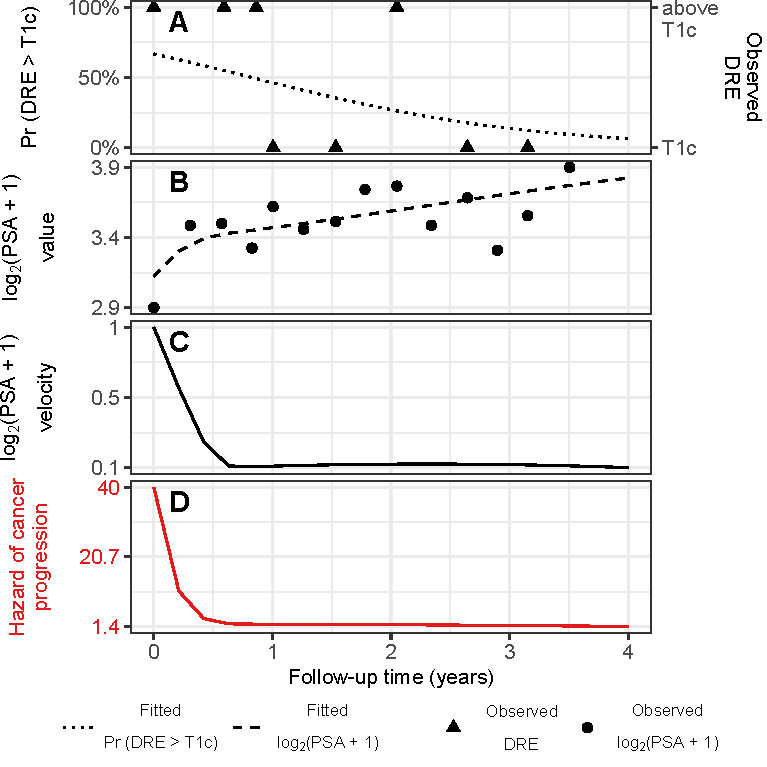
\includegraphics{contents/c3/images/c3_fig3.pdf}
\caption{\textbf{Illustration of the joint model fitted to the PRIAS dataset}. \textbf{Panel~A:} Observed DRE measurements and the fitted probability of obtaining $\mbox{DRE} > \mbox{T1c}$ (\ref{c3:eq:long_model_dre}). \textbf{Panel~B:} Observed and fitted $\log_2(\mbox{PSA} + 1)$ values (\ref{c3:eq:long_model_psa}). \textbf{Panel~C:} Estimated $\log_2(\mbox{PSA} + 1)$ velocity over time. \textbf{Panel~D}: Estimated hazard of cancer progression (\ref{c3:eq:rel_risk_model}). It depends on the fitted log odds of having a $\mbox{DRE} > \mbox{T1c}$, and the fitted $\log_2(\mbox{PSA} + 1)$ value and velocity.}
\label{c3:fig:3}
\end{figure}

In our joint model, the patient-specific DRE and PSA measurements over time are modeled using a bivariate generalized linear mixed effects sub-model. The sub-model for DRE is given by (see~Panel~A, Figure~\ref{c3:fig:3}):
\begin{equation}
\label{c3:eq:long_model_dre}
\begin{split}
    \mbox{logit} \big[\mbox{Pr}\{y_{di}(t) > \mbox{T1c}\}\big] &= \beta_{0d} + b_{0di} + (\beta_{1d} + b_{1di}) t\\
    &+ \beta_{2d} (\mbox{Age}_i-70)  + \beta_{3d} (\mbox{Age}_i-70)^2
    \end{split}
\end{equation}
where, $t$ denotes the follow-up visit time, and $\mbox{Age}_i$ is the age of the ${i\mbox{-th}}$ patient at the time of inclusion in AS. We have centered the Age variable around the median age of 70 years for better convergence during parameter estimation. However, this does not change the interpretation of the parameters corresponding to the Age variable. The fixed effect parameters are denoted by ${\{\beta_{0d}, \ldots, \beta_{3d}\}}$, and ${\{b_{0di}, b_{1di}\}}$ are the patient specific random effects. With this definition, we assume that the patient-specific log odds of obtaining a DRE measurement larger than T1c remain linear over time. 

The mixed effects sub-model for PSA is given by (see~Panel~B, Figure~\ref{c3:fig:3}):
\begin{equation}
\label{c3:eq:long_model_psa}
\begin{split}
    \log_2 \big\{y_{pi}(t) + 1\big\} &= m_{pi}(t) + \varepsilon_{pi}(t),\\
    m_{pi}(t) &= \beta_{0p} + b_{0pi} + \sum_{k=1}^4 (\beta_{kp} + b_{kpi})  B_k(t,\mathcal{K})\\ 
    &+ \beta_{5p} (\mbox{Age}_i-70) + \beta_{6p} (\mbox{Age}_i-70)^2,
    \end{split}
\end{equation}
where, $m_{pi}(t)$ denotes the %underlying
measurement error free value of $\log_2 (\mbox{PSA} + 1)$ transformed~\citep{pearson1994mixed,lin2000latent} measurements at time $t$. We model it non-linearly over time using B-splines~\citep{de1978practical}. To this end, our B-spline basis function $B_k(t, \mathcal{K})$ has 3 internal knots at $\mathcal{K} = \{0.1, 0.7, 4\}$ years, and boundary knots at 0 and 5.42 years (95-th percentile of the observed follow-up times). This specification allows fitting the $\log_2 (\mbox{PSA} + 1)$ levels in a piecewise manner for each patient separately. The internal and boundary knots specify the different time periods (analogously pieces) of this piecewise nonlinear curve. The fixed effect parameters are denoted by ${\{\beta_{0p},\ldots,\beta_{6p}\}}$, and ${\{b_{0pi}, \ldots, b_{4pi}\}}$ are the patient specific random effects. The error $\varepsilon_{pi}(t)$ is assumed to be t-distributed with three degrees of freedom (Figure~\ref{c3:fig:app5}) and scale $\sigma$, and is independent of the random effects. 

To account for the correlation between the DRE and PSA measurements of a patient, we link their corresponding random effects. More specifically, the complete vector of random effects ${\boldsymbol{b}_i = (b_{0di}, b_{1di}, b_{0pi}, \ldots, b_{4pi})^T}$ is assumed to follow a multivariate normal distribution with mean zero and variance-covariance matrix $\boldsymbol{D}$.

To model the impact of DRE and PSA measurements on the risk of cancer progression, our joint model uses a relative risk sub-model. More specifically, the hazard of cancer progression $h_i(t)$ at a time $t$ is given by (see~Panel~D, Figure~\ref{c3:fig:3}):
\begin{equation}
\label{c3:eq:rel_risk_model}
\begin{split}
    h_i(t) &= h_0(t) \exp\Big(\gamma_1 (\mbox{Age}_i-70) + \gamma_2 (\mbox{Age}_i-70)^2\\
    &+\alpha_{1d} \mbox{logit} \big[\mbox{Pr}\{y_{di}(t) > \mbox{T1c}\}\big] + \alpha_{1p} m_{pi}(t) + \alpha_{2p} \frac{\partial m_{pi}(t)}{\partial {t}}\Big),
    \end{split}
\end{equation}
where, $\gamma_1, \gamma_2$ are the parameters for the effect of age. The parameter $\alpha_{1d}$ models the impact of log odds of obtaining a $\mbox{DRE} > \mbox{T1c}$ on the hazard of cancer progression. The impact of PSA on the hazard of cancer progression is modeled in two ways: a) the impact of the error free underlying PSA value $m_{pi}(t)$ (see~Panel~B, Figure~\ref{c3:fig:3}), and b) the impact of the underlying PSA velocity $\partial m_{pi}(t)/\partial {t}$ (see~Panel~C, Figure~\ref{c3:fig:3}). The corresponding parameters are $\alpha_{1p}$ and $\alpha_{2p}$, respectively. Lastly, $h_0(t)$ is the baseline hazard at time $t$, and is modeled flexibly using P-splines~\citep{eilers1996flexible}. More specifically:
\begin{equation*}
\log{h_0(t)} = \gamma_{h_0,0} + \sum_{q=1}^Q \gamma_{h_0,q} B_q(t, \boldsymbol{v}),
\end{equation*}
where $B_q(t, \boldsymbol{v})$ denotes the $q$-th basis function of a B-spline with knots $\boldsymbol{v} = v_1, \ldots, v_Q$ and vector of spline coefficients $\gamma_{h_0}$. To avoid choosing the number and position of knots in the spline, a relatively high number of knots (e.g., 15 to 20) are chosen and the corresponding B-spline regression coefficients $\gamma_{h_0}$ are penalized using a differences penalty~\citep{eilers1996flexible}.The detailed specification of the baseline hazard $h_0(t)$, and the joint parameter estimation of the two sub-models using the Bayesian approach (R package \textbf{JMbayes}) are presented in Appendix~\ref{c3:appendix:A}.

\subsection{Personalized Decisions for Biopsy}
\label{c3:subsec:pers_decision_making}
Let us assume that a decision of conducting a biopsy is to be made for a new patient $j$ shown in Figure~\ref{c3:fig:1}, at his current follow-up visit time $s$. Let $t\leq s$ be the time of his latest negative biopsy. Let $\mathcal{Y}_{dj}(s)$ and $\mathcal{Y}_{pj}(s)$ denote his observed DRE and PSA measurements up to the current visit, respectively. From the observed measurements we want to extract the underlying measurement error free trend of $\log_2 (\mbox{PSA} + 1)$ values and velocity, and the log odds of obtaining $\mbox{DRE} > \mbox{T1c}$. We intend to combine them to inform us when the cancer progression is to be expected, and to further guide the decision making on whether to conduct a biopsy at the current follow-up visit. The combined information is given by the following posterior predictive distribution $g(T^*_j)$ of his time of cancer progression $T^*_j > t$:
\begin{equation}
\label{c3:eq:post_pred_dist}
g(T^*_j) = p\big\{T^*_j \mid T^*_j > t, \mathcal{Y}_{dj}(s), \mathcal{Y}_{pj}(s), \mathcal{D}_n\big\}.
\end{equation}
The distribution $g(T^*_j)$ is not only patient-specific, but also updates as extra information is recorded at future follow-up visits.

\begin{figure}
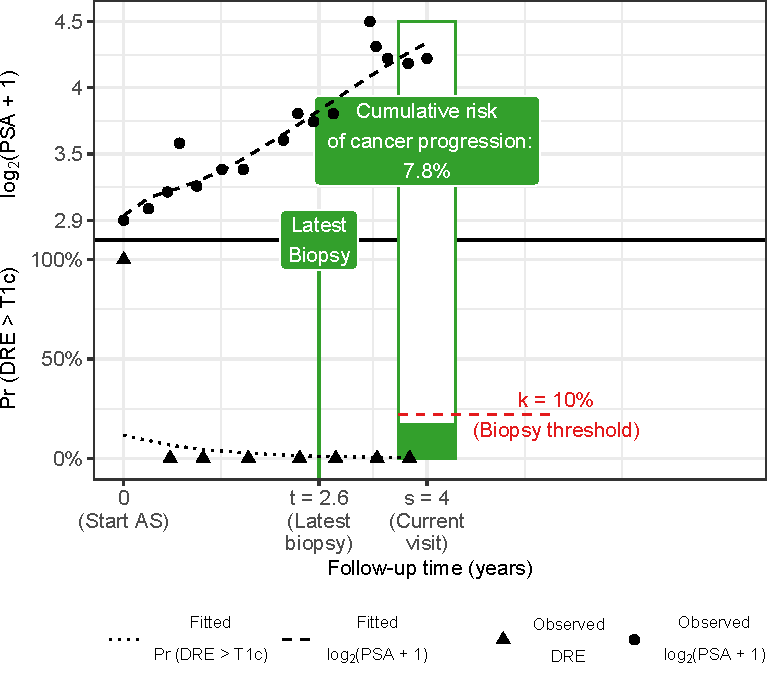
\includegraphics{contents/c3/images/c3_fig4a.pdf}
\caption{\textbf{Personalized decision biopsy not recommended}: Biopsy is recommended only if the personalized cumulative-risk of cancer progression estimated from the joint model fitted to the observed data of the $j$-th patient, is higher than the example risk threshold for biopsy ($\kappa=$ 10\%). The cumulative-risk of cancer progression at the current visit time ($s=$ 4 years) is 7.8\%.}
\label{c3:fig:4a}
\end{figure}

\begin{figure}
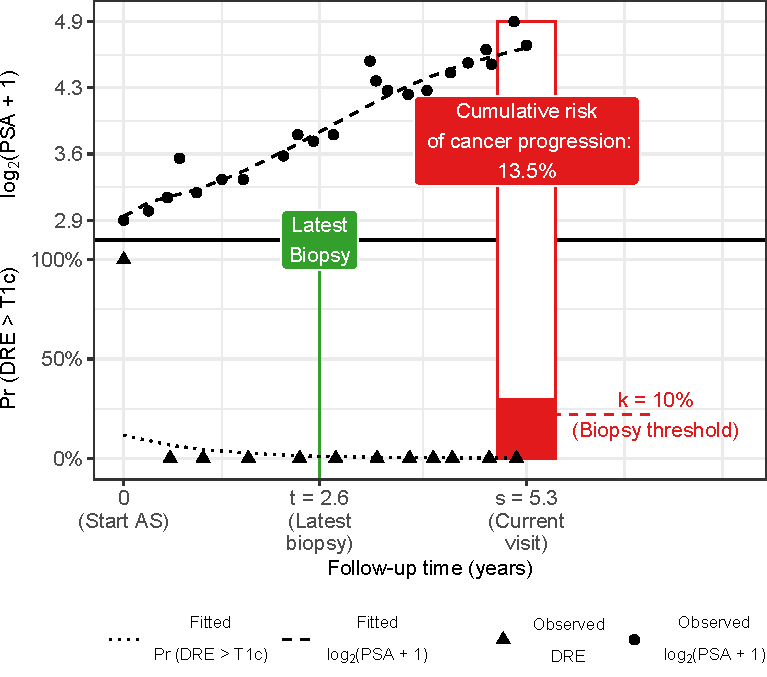
\includegraphics{contents/c3/images/c3_fig4b.pdf}
\caption{\textbf{Personalized decision of biopsy recommended}: Biopsy is recommended only if the personalized cumulative-risk of cancer progression estimated from the joint model fitted to the observed data of the $j$-th patient, is higher than the example risk threshold for biopsy ($\kappa=$ 10\%). The cumulative-risk of cancer progression at the current visit time ($s=$ 5.3 years) is 13.5\%.}
\label{c3:fig:4b}
\end{figure}

A key ingredient in the decision of conducting a biopsy for patient $j$ at the current follow-up visit time $s$ is the personalized cumulative-risk of observing a cancer progression at time $s$ (illustrated in Figure~\ref{c3:fig:4a}, and Figure~\ref{c3:fig:4b}). This risk can be derived from the posterior predictive distribution $g(T^*_j)$~\citep{rizopoulos2011dynamic}, and for $s \geq t$ it is given by:
\begin{equation}
\label{c3:eq:dynamic_risk_prob}
R_j(s \mid t) = \mbox{Pr}\big\{T^*_j \leq s \mid T^*_j > t, \mathcal{Y}_{dj}(s), \mathcal{Y}_{pj}(s), \mathcal{D}_n\big\}.
\end{equation}
A simple and straightforward approach to decide upon conducting a biopsy for patient $j$ at the current follow-up visit would be to do so if his personalized cumulative-risk of cancer progression at the visit is higher than a certain threshold $0 \leq \kappa \leq 1$. For example, as shown in Figure~\ref{c3:fig:4a}, and Figure~\ref{c3:fig:4b}, biopsy at a visit may be scheduled if the personalized cumulative-risk is higher than 10\% (example risk threshold). This decision making process is iterated over the follow-up period, incorporating on each subsequent visit the newly observed data, until a positive biopsy is observed. Subsequently, an entire personalized schedule of biopsies for each patient can be obtained.

The choice of the risk threshold dictates the schedule of biopsies and has to be made on each subsequent follow-up visit of a patient. In this regard, a straightforward approach is choosing a fixed risk threshold, such as 5\% or 10\% risk, at all follow-up visits. Fixed risk thresholds may be chosen by patients and/or doctors according to how they weigh the relative harms of doing an unnecessary biopsy versus a missed cancer progression (e.g., 10\% threshold means a 1:9 ratio) if the biopsy is not conducted~\citep{vickers2006decision}. An alternative approach is that at each follow-up visit, a unique threshold is chosen on the basis of its classification accuracy. More specifically, given the time of latest biopsy $t$ of patient $j$, and his current visit time $s$\, we find a visit-specific biopsy threshold $\kappa$, which gives the highest cancer progression detection rate (true positive rate, or TPR) for the period $(t, s]$. However, we also intend to balance for unnecessary biopsies (high false-positive rate), or a low number of correct detections (high false-negative rate) when the false positive rate is minimized. An approach to mitigating these issues is to maximize the TPR and positive predictive value (PPV) simultaneously. To this end, we utilize the $\mbox{F}_1$~score, which is a composite of both TPR and PPV [estimated as in~\citet{landmarking2017}] and is defined as: 
\begin{equation}
\label{c3:eq:F1_TPR_PPV}
\begin{split}
\mbox{F}_1(t,  s, \kappa) &= 2\frac{\mbox{TPR}(t,  s, \kappa)\ \mbox{PPV}(t,  s, \kappa)}{\mbox{TPR}(t,  s, \kappa) + \mbox{PPV}(t,  s, \kappa)},\\
\mbox{TPR}(t,  s, \kappa) &= \mbox{Pr}\big\{R_j(s \mid t) > \kappa \mid t < T^*_j \leq s\big\},\\
\mbox{PPV}(t,  s, \kappa) &= \mbox{Pr}\big\{t < T^*_j \leq s \mid R_j(s \mid t) > \kappa \big\},
\end{split}
\end{equation}
where, $\mbox{TPR}(t,  s, \kappa)$ and $\mbox{PPV}(t,  s, \kappa)$ are the time-dependent true positive rate and positive predictive value, respectively. These values are unique for each combination of the time period $(t, s]$ and the risk threshold $\kappa$ that is used to discriminate between the patients whose cancer progresses in this time period versus the patients whose cancer does not progress. The same holds true for the resulting $\mbox{F}_1$~score denoted by $\mbox{F}_1(t,  s, \kappa)$. The $\mbox{F}_1$~score ranges between 0 and 1, where a value equal to 1 indicates perfect TPR and PPV. Thus the highest $\mbox{F}_1$~score is desired in each time period $(t, s]$. This can be achieved by choosing a risk threshold $\kappa$, which maximizes $\mbox{F}_1(t, s, \kappa)$. That is, during a patient's visit at time $s$, given that his latest biopsy was at the time $t$, the visit-specific risk threshold to decide a biopsy is given by ${\kappa=\argmax_{\kappa} \mbox{F}_1(t, s, \kappa)}$. The criteria on which we evaluate the personalized schedules based on fixed and visit-specific risk thresholds is the total number of biopsies scheduled, and the delay in detection of cancer progression (details in \hyperref[sec:results]{Results}). 

\subsection{Simulation Study}
\label{c3:subsec:sim_study}
Although the personalized decision-making approach is motivated by the PRIAS study, it is not possible to evaluate it directly on the PRIAS dataset. This is because the patients in PRIAS have already had their biopsies as per the PRIAS protocol. In addition, the true time of cancer progression is interval or right-censored for all patients, making it impossible to correctly estimate the delay in the detection of cancer progression due to a particular schedule. To this end, we conduct an extensive simulation study to find the utility of personalized, PRIAS, and fixed/heuristic schedules. For a realistic comparison, we simulate patient data from the joint model fitted to the PRIAS dataset. The simulated population has the same ten year follow-up period as the PRIAS study. In addition, the estimated relations between DRE and PSA measurements, and the risk of cancer progression are retained in the simulated population.

From this population, we first sample 500 datasets, each representing a hypothetical AS program with 1000 patients in it. We generate a true cancer progression time for each of the ${\mbox{500} \times \mbox{1000}}$ patients and then sample a set of DRE and PSA measurements at the same follow-up visit times as given in PRIAS protocol. We then split each dataset into training (750 patients) and test (250 patients) parts, and generate a random and non-informative censoring time for the training patients. We next fit a joint model of the specification given in~(\ref{c3:eq:long_model_dre}),~(\ref{c3:eq:long_model_psa}),~and~(\ref{c3:eq:rel_risk_model}) to each of the 500 training datasets and obtain MCMC samples from the 500 sets of the posterior distribution of the parameters. 

In each of the 500 hypothetical AS programs, we utilize the corresponding fitted joint models to develop cancer progression risk profiles for each of the ${\mbox{500} \times \mbox{250}}$ test patients. We make the decision of biopsies for patients at their pre-scheduled follow-up visits for DRE and PSA measurements (see Section~\ref{c3:subsec:study_population}), on the basis of their estimated personalized cumulative-risk of cancer progression. These decisions are made iteratively until a positive biopsy is observed. A recommended gap of one year between consecutive biopsies~\citep{bokhorst2015compliance} is also maintained. Subsequently, for each patient, an entire personalized schedule of biopsies is obtained.

We evaluate and compare both personalized and currently practiced schedules of biopsies in this simulation study. A comparison of the schedules is based on the number of biopsies scheduled and the corresponding delay in the detection of cancer progression. We evaluate the following currently practiced fixed/heuristic schedules: biopsy annually, biopsy every one and a half years, biopsy every two years, and biopsy every three years. We also evaluate the biopsy schedule of the PRIAS program (see Section~\ref{c3:sec:introduction}). For the personalized biopsy schedules, we evaluate schedules based on three fixed risk thresholds: 5\%, 10\%, and 15\%, corresponding to a missed cancer progression being 19, 9, and 5.5 times more harmful than an unnecessary biopsy~\citep{vickers2006decision}, respectively. We also implement a personalized schedule wherein for each patient, visit-specific risk thresholds are chosen using $\mbox{F}_1$~score.